\documentclass[pdftex,12pt,a4paper]{report}

\usepackage[portuguese,english]{babel}
\usepackage[T1]{fontenc} 
\usepackage[table]{xcolor}
\usepackage[utf8]{inputenc}
\usepackage[pdftex]{graphicx}
\usepackage{minitoc}
\usepackage{hyperref}
\usepackage{indentfirst}
\usepackage[compact]{titlesec}
\usepackage{fancyhdr}
\usepackage{caption}
\usepackage{pgfplots}
\usepackage{pgfplotstable}
\usepackage{fixltx2e}
\usepackage{mathtools}
\usepackage{fancyhdr}
\usepackage{listings}
\usepackage{color}
\usepackage{sverb}
\usepackage[section]{placeins}

%Highlight
\newcommand{\shellcmd}[1]{\indent\indent\texttt{\footnotesize\# #1}\\}

\pagestyle{fancy}
\renewcommand*\thesection{\thechapter\arabic{section}}
\newcommand{\HRule}{\rule{\linewidth}{0.5mm}}
\begin{document}

\begin{titlepage}

\begin{center}


\includegraphics[width=0.15\textwidth]{./logo}\\[0.5cm]    

\textsc{\large Universidade de Aveiro \\[1cm]\large departamento de electrónica, telecomunicações e informática}\\[1cm]

\textsc{\large Gestão Integrada de Redes e Sistemas\\[1cm]}

\HRule \\[0.5cm]
{ \huge \bfseries RAID, NAS and SAN}\\[0.4cm]
{ \large \bfseries Exercício Prático}\\[0.4cm]
\HRule \\[1cm]

\textsc{\small{8240 - MESTRADO INTEGRADO EM ENGENHARIA DE COMPUTADORES E TELEMÁTICA}}\\[1cm]

\begin{minipage}{0.4\textwidth}

\begin{flushleft} \large
\href{mailto:rafael.ferreira@ua.pt}{António Rafael da \\ Costa Ferreira }
 \small{\\NMec: 67405}
\end{flushleft}
\end{minipage}
\begin{minipage}{0.4\textwidth}

\begin{flushright} \large
\href{mailto:rodrigocunha@ua.pt}{Rodrigo Lopes \\ da Cunha}
\small{\\NMec: 67800}
\end{flushright}
\end{minipage}\\[1cm]

{\large Docentes: Diogo Gomes,}\\
{\large \hspace{2.5cm} João Paulo Barraca}\\[0.5cm]


\vfill

{\large Março de 2016 \\ 2015-2016}

\end{center}

\end{titlepage} %Titulo do Relatorio
\renewcommand{\headrulewidth}{0pt}

%Cabeçalhos de rodapé
\fancyhead{}
\fancyfoot{}
\lhead{Storage}
\rhead{GIRS - 2015/2016}
\lfoot{Rafael Ferreira nmec: 67405 \\ Rodrigo Cunha nmec: 67800}
\rfoot{\thepage}

%Renomear Comandos
\renewcommand*\contentsname{Conteúdos}
\renewcommand*\figurename{Figura}
\renewcommand*\tablename{Tabela}

%Conteúdos, dar paragrafo
\tableofcontents
%Headers
\renewcommand{\headrulewidth}{0.15pt}
\renewcommand{\thechapter}{}

\clearpage

\section{RAID}

\subsection{Criação de um RAID}

\subsection{Configuração}

\begin{figure}[!htb]
\center
 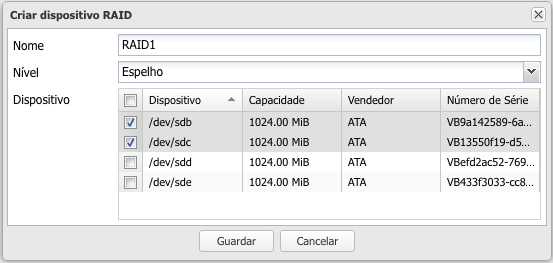
\includegraphics[width=150mm,scale=1]{imagens/RAID1Create.png}
 \caption{RAID 1}
 \label{fig:exemploraid}
\end{figure}

Para se avaliar os diferentes níveis de RAID usou-se o OpenMediaVault que é um sistema operativo para gestão de um NAS baseado em Debian (Linux).

Para instalação do ambiente foi criado uma máquina virtual usando a Virtual Box com 4 discos com 1024MB.

Depois foi criado diferentes níveis de RAID, sendo estes o nível 0, 1, 5, 6 e 10. Observou-se para os diferentes níveis de RAID qual é o espaço disponível e removendo os discos qual é o número de falhas que podem existir para que os dados não sejam perdidos. 

\begin{table}[!htb]
\centering
\caption{Avaliação dos diferentes níveis de RAID}
\label{my-label}
\begin{tabular}{|c|c|c|c|}
\hline
\multicolumn{1}{|l|}{\textbf{RAID}} & \multicolumn{1}{l|}{\textbf{Número de discos}} & \multicolumn{1}{l|}{\textbf{Espaço disponível}} & \multicolumn{1}{l|}{\textbf{Número de falhas permitidas}} \\ \hline
0                                   & 2                                              & 2 GB                                            & 0                                                        \\ \hline
1                                   & 2                                              & 1023.44 MB                                      & 1 (N-1)                                                  \\ \hline
10                                  & 4                                              & 2 GB                                            & 2 (N/2)                                                  \\ \hline
5                                   & 3                                              & 2 GB                                            & 1                                                        \\ \hline
6                                   & 4                                              & 2 GB                                            & 1                                                        \\ \hline
\end{tabular}
\end{table}

\section{NAS/SAN}

\subsection{Configuração do NAS}

Na segunda parte do trabalho foi-nos pedido que fosse feito uma NAS/SAN, para isso começou-se por criar um RAID 0 e criou-se um volume com o RAID 0 criado com o nome "md1" com o sistema de ficheiros "ext3". 

\begin{figure}[!htb]
\center
 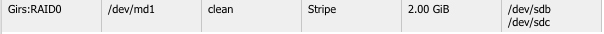
\includegraphics[width=150mm,scale=1]{imagens/RAID0.png}
 \caption{RAID 0}
 \label{fig:raid0}
\end{figure}

\begin{figure}[!htb]
\center
 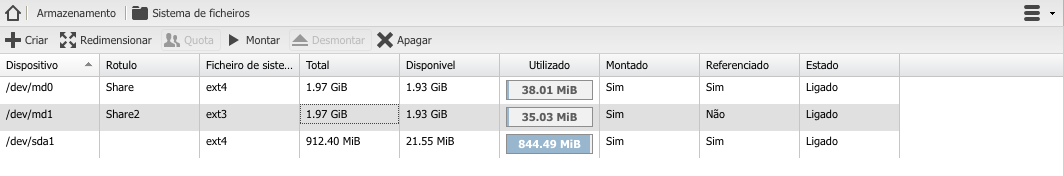
\includegraphics[width=150mm,scale=1]{imagens/FileSystem.png}
 \caption{Volume "md1"}
 \label{fig:exemploraid}
\end{figure}

Usando o Samba fez-se partilha do novo Volume criado como mostra a figura \ref{fig:SharedFolders}.

\begin{figure}[!htb]
\center
 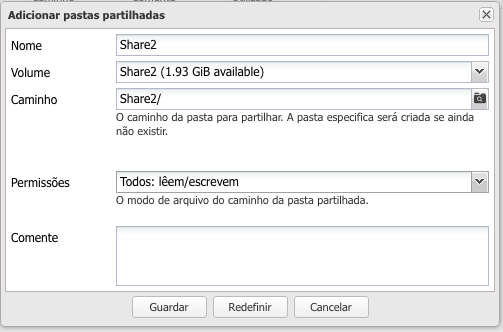
\includegraphics[width=100mm,scale=1]{imagens/AddShare2.png}
 \caption{Adicionar o Volume para partilha}
 \label{fig:SharedFolders}
\end{figure}

Depois montou-se a pasta partilhada como sendo um NAS num OS X como demonstra a figura \ref{fig:MacSharedFolders}.

\begin{figure}[!htb]
\center
 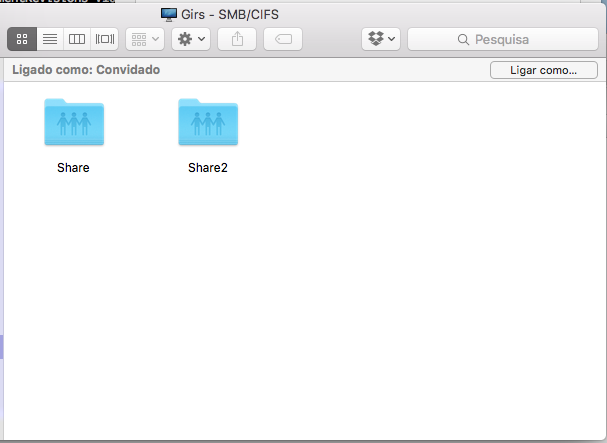
\includegraphics[width=80mm,scale=1]{imagens/MacSharedFolders.png}
 \caption{Pastas partilhadas}
 \label{fig:MacSharedFolders}
\end{figure}

\subsection{Teste do NAS}

Para testar se realmente estaria ou não a funcionar o NAS criado, criou-se um ficheiro na máquina virtual como demonstra a figura \ref{fig:CreateTestVM}.

\begin{figure}[!htb]
\center
 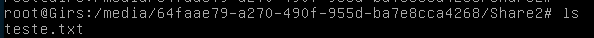
\includegraphics[width=80mm,scale=1]{imagens/CreateTestVM.png}
 \caption{Adicionar o Volume para partilha}
 \label{fig:CreateTestVM}
\end{figure}

Após isso, verificou-se se no OS X o ficheiro também já existia, e de facto, existia, como demonstra a figura \ref{fig:testMac.png}.

\subsection{Benchmark do NAS Volume}

Usando o "bonnie++" efetuou-se 10 medições e calculou-se a média para obter resultados finais para a experiência, como mostra as tabelas \ref{table:bonnie++1}, \ref{table:bonnie++2} e \ref{table:bonnie++3}.

% Please add the following required packages to your document preamble:
% \usepackage[table,xcdraw]{xcolor}
% If you use beamer only pass "xcolor=table" option, i.e. \documentclass[xcolor=table]{beamer}
\begin{table}[!htb]
\centering
\caption{Resultados do benchmark usando bonnie++ (Parte 1)}
\label{table:bonnie++1}
\resizebox{\textwidth}{!}{\begin{tabular}{l|c|c|c|c|c|c|}
\cline{2-7}
                                                            & \cellcolor[HTML]{FFCC67}\textbf{Bonnie++ Version} & \cellcolor[HTML]{FFCC67}\textbf{Concurrency Level} & \cellcolor[HTML]{FFCC67}\textbf{Random Number Seed} & \cellcolor[HTML]{FFCC67}\textbf{File Size} & \cellcolor[HTML]{FFCC67}\textbf{Block Writes (K/s)} & \cellcolor[HTML]{FFCC67}\textbf{(\% cpu)} \\ \cline{2-7} 
                                                            & 1.97                                              & 1                                                  & 1459450816                                          & 8G                                         & 88149                                               & 10                                        \\ \cline{2-7} 
                                                            & 1.97                                              & 1                                                  & 1459453831                                          & 8G                                         & 72789                                               & 6                                         \\ \cline{2-7} 
                                                            & 1.97                                              & 1                                                  & 1459452397                                          & 8G                                         & 73546                                               & 7                                         \\ \cline{2-7} 
                                                            & 1.97                                              & 1                                                  & 1459452673                                          & 8G                                         & 75701                                               &                                           \\ \cline{2-7} 
                                                            & 1.97                                              & 1                                                  & 1459447167                                          & 8G                                         & 88738                                               & 9                                         \\ \cline{2-7} 
                                                            & 1.97                                              & 1                                                  & 1459446918                                          & 8G                                         & 72541                                               & 7                                         \\ \cline{2-7} 
                                                            & 1.97                                              & 1                                                  & 1459445918                                          & 8G                                         & 78299                                               & 7                                         \\ \cline{2-7} 
                                                            & 1.97                                              & 1                                                  & 1459449549                                          & 8G                                         & 75141                                               & 7                                         \\ \cline{2-7} 
                                                            & 1.97                                              & 1                                                  & 1459449100                                          & 8G                                         & 75521                                               & 7                                         \\ \cline{2-7} 
                                                            & 1.97                                              & 1                                                  & 1459449032                                          & 8G                                         & 80327                                               & 8                                         \\ \hline
\rowcolor[HTML]{FFFC9E} 
\multicolumn{1}{|c|}{\cellcolor[HTML]{F8A102}\textbf{média}} & {\color[HTML]{333333} \textbf{1.97}}              & {\color[HTML]{333333} \textbf{1}}                  & {\color[HTML]{333333} \textbf{1459449740}}          & {\color[HTML]{333333} \textbf{8G}}         & {\color[HTML]{333333} \textbf{78075,2}}             & {\color[HTML]{333333} \textbf{7,5}}       \\ \hline
\end{tabular}}
\end{table}


% Please add the following required packages to your document preamble:
% \usepackage[table,xcdraw]{xcolor}
% If you use beamer only pass "xcolor=table" option, i.e. \documentclass[xcolor=table]{beamer}
\begin{table}[!htb]
\centering
\caption{Resultados do benchmark usando bonnie++ (Parte 2)}
\label{table:bonnie++2}
\resizebox{\textwidth}{!}{\begin{tabular}{l|c|c|c|c|c|c|}
\cline{2-7}
                                                            & \cellcolor[HTML]{FFCC67}\textbf{Reading/Rewriting Block (K/s)} & \cellcolor[HTML]{FFCC67}\textbf{(\% cpu)} & \cellcolor[HTML]{FFCC67}\textbf{Block Reads (K/s)} & \cellcolor[HTML]{FFCC67}\textbf{(\% cpu)} & \cellcolor[HTML]{FFCC67}\textbf{Seek (s/s)} & \cellcolor[HTML]{FFCC67}\textbf{(\% cpu)} \\ \cline{2-7} 
                                                            & 21758                                                          & 6                                         & 47470                                              & 5                                         & 1000                                        & 31                                        \\ \cline{2-7} 
                                                            & 32983                                                          & 5                                         & 77413                                              & 8                                         & 940,2                                       & 27                                        \\ \cline{2-7} 
                                                            & 38005                                                          & 6                                         & 77339                                              & 7                                         & 1103                                        & 35                                        \\ \cline{2-7} 
                                                            & 30252                                                          & 6                                         & 71017                                              & 7                                         & 1060                                        & 35                                        \\ \cline{2-7} 
                                                            & 32433                                                          & 10                                        & 73999                                              & 7                                         & 1055                                        & 33                                        \\ \cline{2-7} 
                                                            & 36601                                                          & 6                                         & 74004                                              & 7                                         & 1004                                        & 32                                        \\ \cline{2-7} 
                                                            & 32597                                                          & 6                                         & 66784                                              & 7                                         & 1093                                        & 34                                        \\ \cline{2-7} 
                                                            & 31529                                                          & 6                                         & 71241                                              & 7                                         & 907,1                                       & 29                                        \\ \cline{2-7} 
                                                            & 33710                                                          & 6                                         & 74052                                              & 7                                         & 994,8                                       & 31                                        \\ \cline{2-7} 
                                                            & 32089                                                          & 5                                         & 73297                                              & 7                                         & 973,5                                       & 31                                        \\ \hline
\rowcolor[HTML]{FFFC9E} 
\multicolumn{1}{|c|}{\cellcolor[HTML]{F8A102}\textbf{média}} & {\color[HTML]{333333} \textbf{32195,7}}                        & {\color[HTML]{333333} \textbf{6,2}}       & {\color[HTML]{333333} \textbf{70661,6}}            & {\color[HTML]{333333} \textbf{6,9}}       & {\color[HTML]{333333} \textbf{1013,06}}     & {\color[HTML]{333333} \textbf{31,8}}      \\ \hline
\end{tabular}}
\end{table}

% Please add the following required packages to your document preamble:
% \usepackage[table,xcdraw]{xcolor}
% If you use beamer only pass "xcolor=table" option, i.e. \documentclass[xcolor=table]{beamer}
\begin{table}[!htb]
\centering
\caption{Resultados do benchmark usando bonnie++ (Parte 3)}
\label{table:bonnie++3}
\resizebox{\textwidth}{!}{\begin{tabular}{l|c|c|c|l|}
\cline{2-5}
                                                            & \cellcolor[HTML]{FFCC67}\textbf{Block Write Latency (ms)} & \cellcolor[HTML]{FFCC67}\textbf{Rewrite Latency (ms)} & \cellcolor[HTML]{FFCC67}\textbf{Block Read Latency (ms)} & \cellcolor[HTML]{FFCC67}\textbf{Seek Latency (ms)} \\ \cline{2-5} 
                                                            & 4009                                                      & 11369                                                 & 11902                                                    & 175                                                \\ \cline{2-5} 
                                                            & 27544                                                     & 11565                                                 & 10906                                                    & 3186                                               \\ \cline{2-5} 
                                                            & 5024                                                      & 25956                                                 & 11947                                                    & 1697                                               \\ \cline{2-5} 
                                                            & 5512                                                      & 10859                                                 & 9862                                                     & 168                                                \\ \cline{2-5} 
                                                            & 4185                                                      & 21276                                                 & 10784                                                    & 2173                                               \\ \cline{2-5} 
                                                            & 4909                                                      & 12442                                                 & 11381                                                    & 2292                                               \\ \cline{2-5} 
                                                            & 5541                                                      & 10699                                                 & 11237                                                    & 178                                                \\ \cline{2-5} 
                                                            & 6399                                                      & 11024                                                 & 11982                                                    & 169                                                \\ \cline{2-5} 
                                                            & 5440                                                      & 11958                                                 & 13269                                                    & 171                                                \\ \cline{2-5} 
                                                            & 4428                                                      & 34282                                                 & 11390                                                    & 182                                                \\ \hline
\rowcolor[HTML]{FFFC9E} 
\multicolumn{1}{|c|}{\cellcolor[HTML]{F8A102}\textbf{média}} & {\color[HTML]{333333} \textbf{7299,1}}                    & {\color[HTML]{333333} \textbf{16143}}                 & {\color[HTML]{333333} \textbf{11466}}                    & {\color[HTML]{333333} \textbf{1039,1}}             \\ \hline
\end{tabular}}
\end{table}

\newpage

No final concluiu-se que para o mesmo nível de concorrência e para a escrita e leitura de um ficheiro com o tamanho de 8GB que: 

% Please add the following required packages to your document preamble:
% \usepackage[table,xcdraw]{xcolor}
% If you use beamer only pass "xcolor=table" option, i.e. \documentclass[xcolor=table]{beamer}
\begin{table}[!htb]
\centering
\caption{Resultados finais da benchmark bonnie++}
\label{table:resultados_bonnie}
\resizebox{\textwidth}{!}{\begin{tabular}{|
>{\columncolor[HTML]{FFCE93}}l |c|
>{\columncolor[HTML]{FFCE93}}l |c|}
\hline
\textbf{Block Writes (K/s)}            & 78075,2 & \textbf{Seek (s/s)}               & 1013,06 \\ \hline
\textbf{(\% cpu)}                      & 7,5     & \textbf{(\% cpu)}                 & 31,8    \\ \hline
\textbf{Reading/Rewriting Block (K/s)} & 32195,7 & \textbf{Block Write Latency (ms)} & 7299,1  \\ \hline
\textbf{(\% cpu)}                      & 6,2     & \textbf{Rewrite Latency (ms)}     & 16143   \\ \hline
\textbf{Block Reads (K/s)}             & 70661,6 & \textbf{Block Read Latency (ms)}  & 11466   \\ \hline
\textbf{(\% cpu)}                      & 6,9     & \textbf{Seek Latency (ms)}        & 1039,1  \\ \hline
\end{tabular}}
\end{table}


\end{document}

